\documentclass[]{article}
\usepackage{graphicx}
\usepackage[margin=1cm]{geometry}
\usepackage{csvsimple}

\begin{document}
\section*{\centering $ 0.3 < p_T < 1.5$ and $ |\eta|<1$}
\subsubsection*{\centering N NPOMS and all NPOMH}
\begin{figure}[h!]
\centering
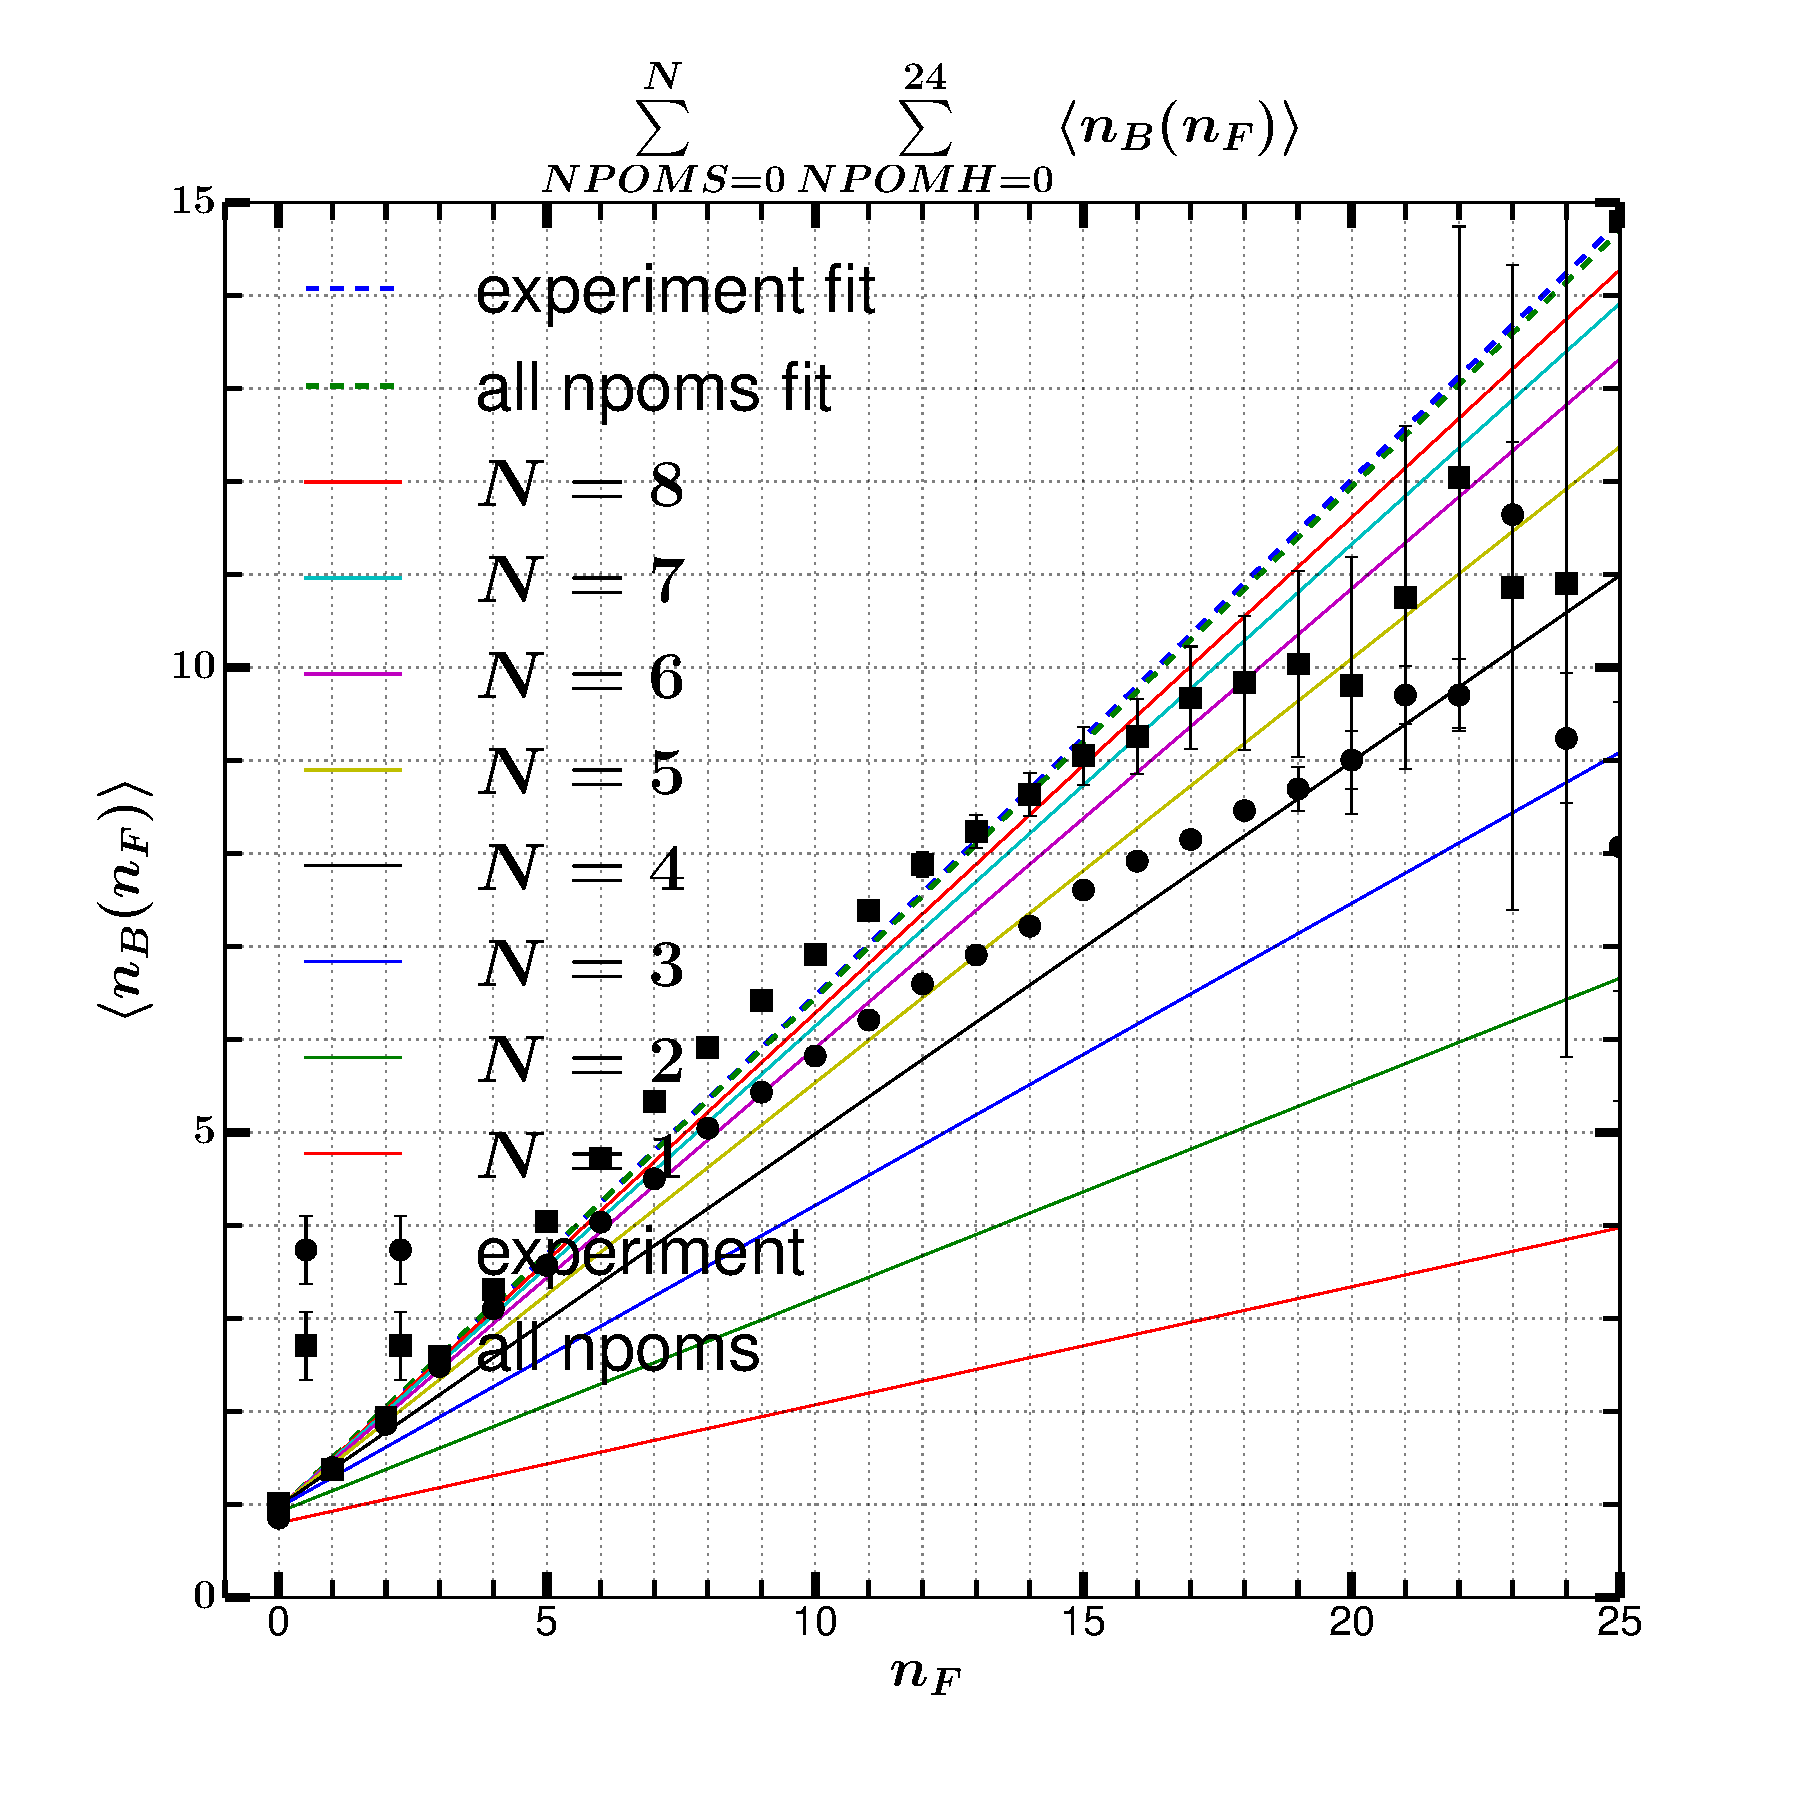
\includegraphics[scale=0.5]{../analyzed/nbnf_Nnpoms_allnpomh.pdf}
\caption{}
\end{figure}

\begin{center}
\csvautotabular{../analyzed/fits.csv}
\end{center}

\newpage
\subsubsection*{\centering All NPOMS and NPOMH=0}

\begin{figure}[h!]
    \centering
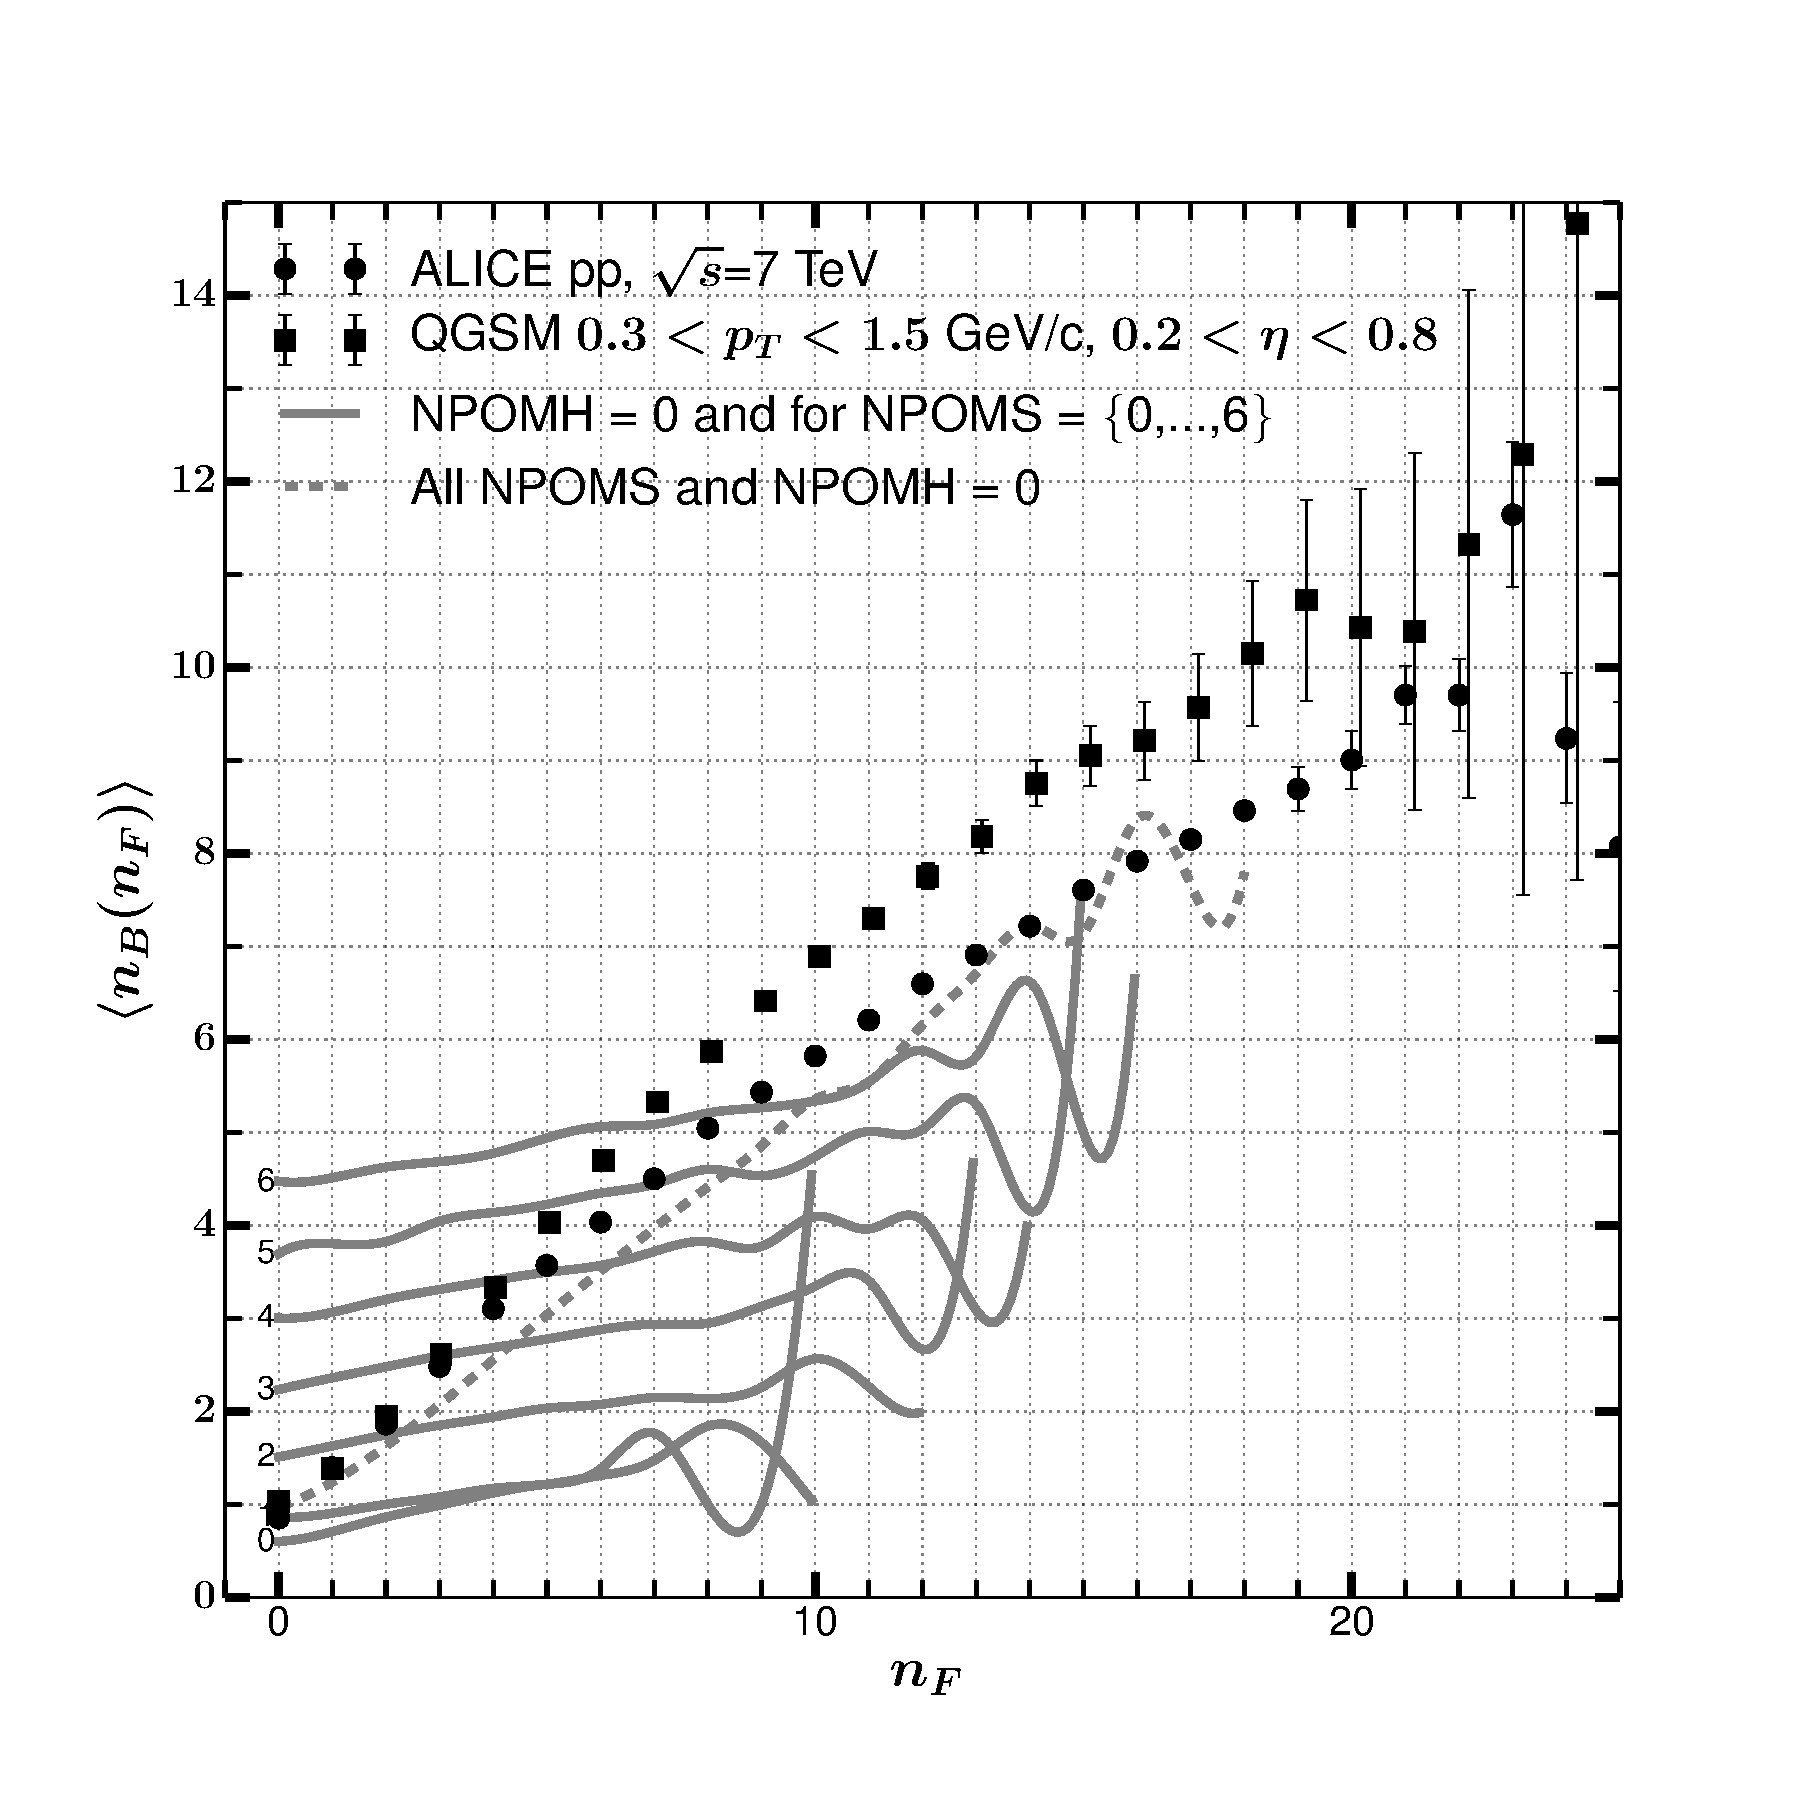
\includegraphics[scale=0.5]{../analyzed/nbnf_allnpoms_0npomh.pdf}
\caption{}
\end{figure}

\subsubsection*{\centering Fixed NPOMS and varying NPOMH}

\begin{figure}[h!]
    \centering
    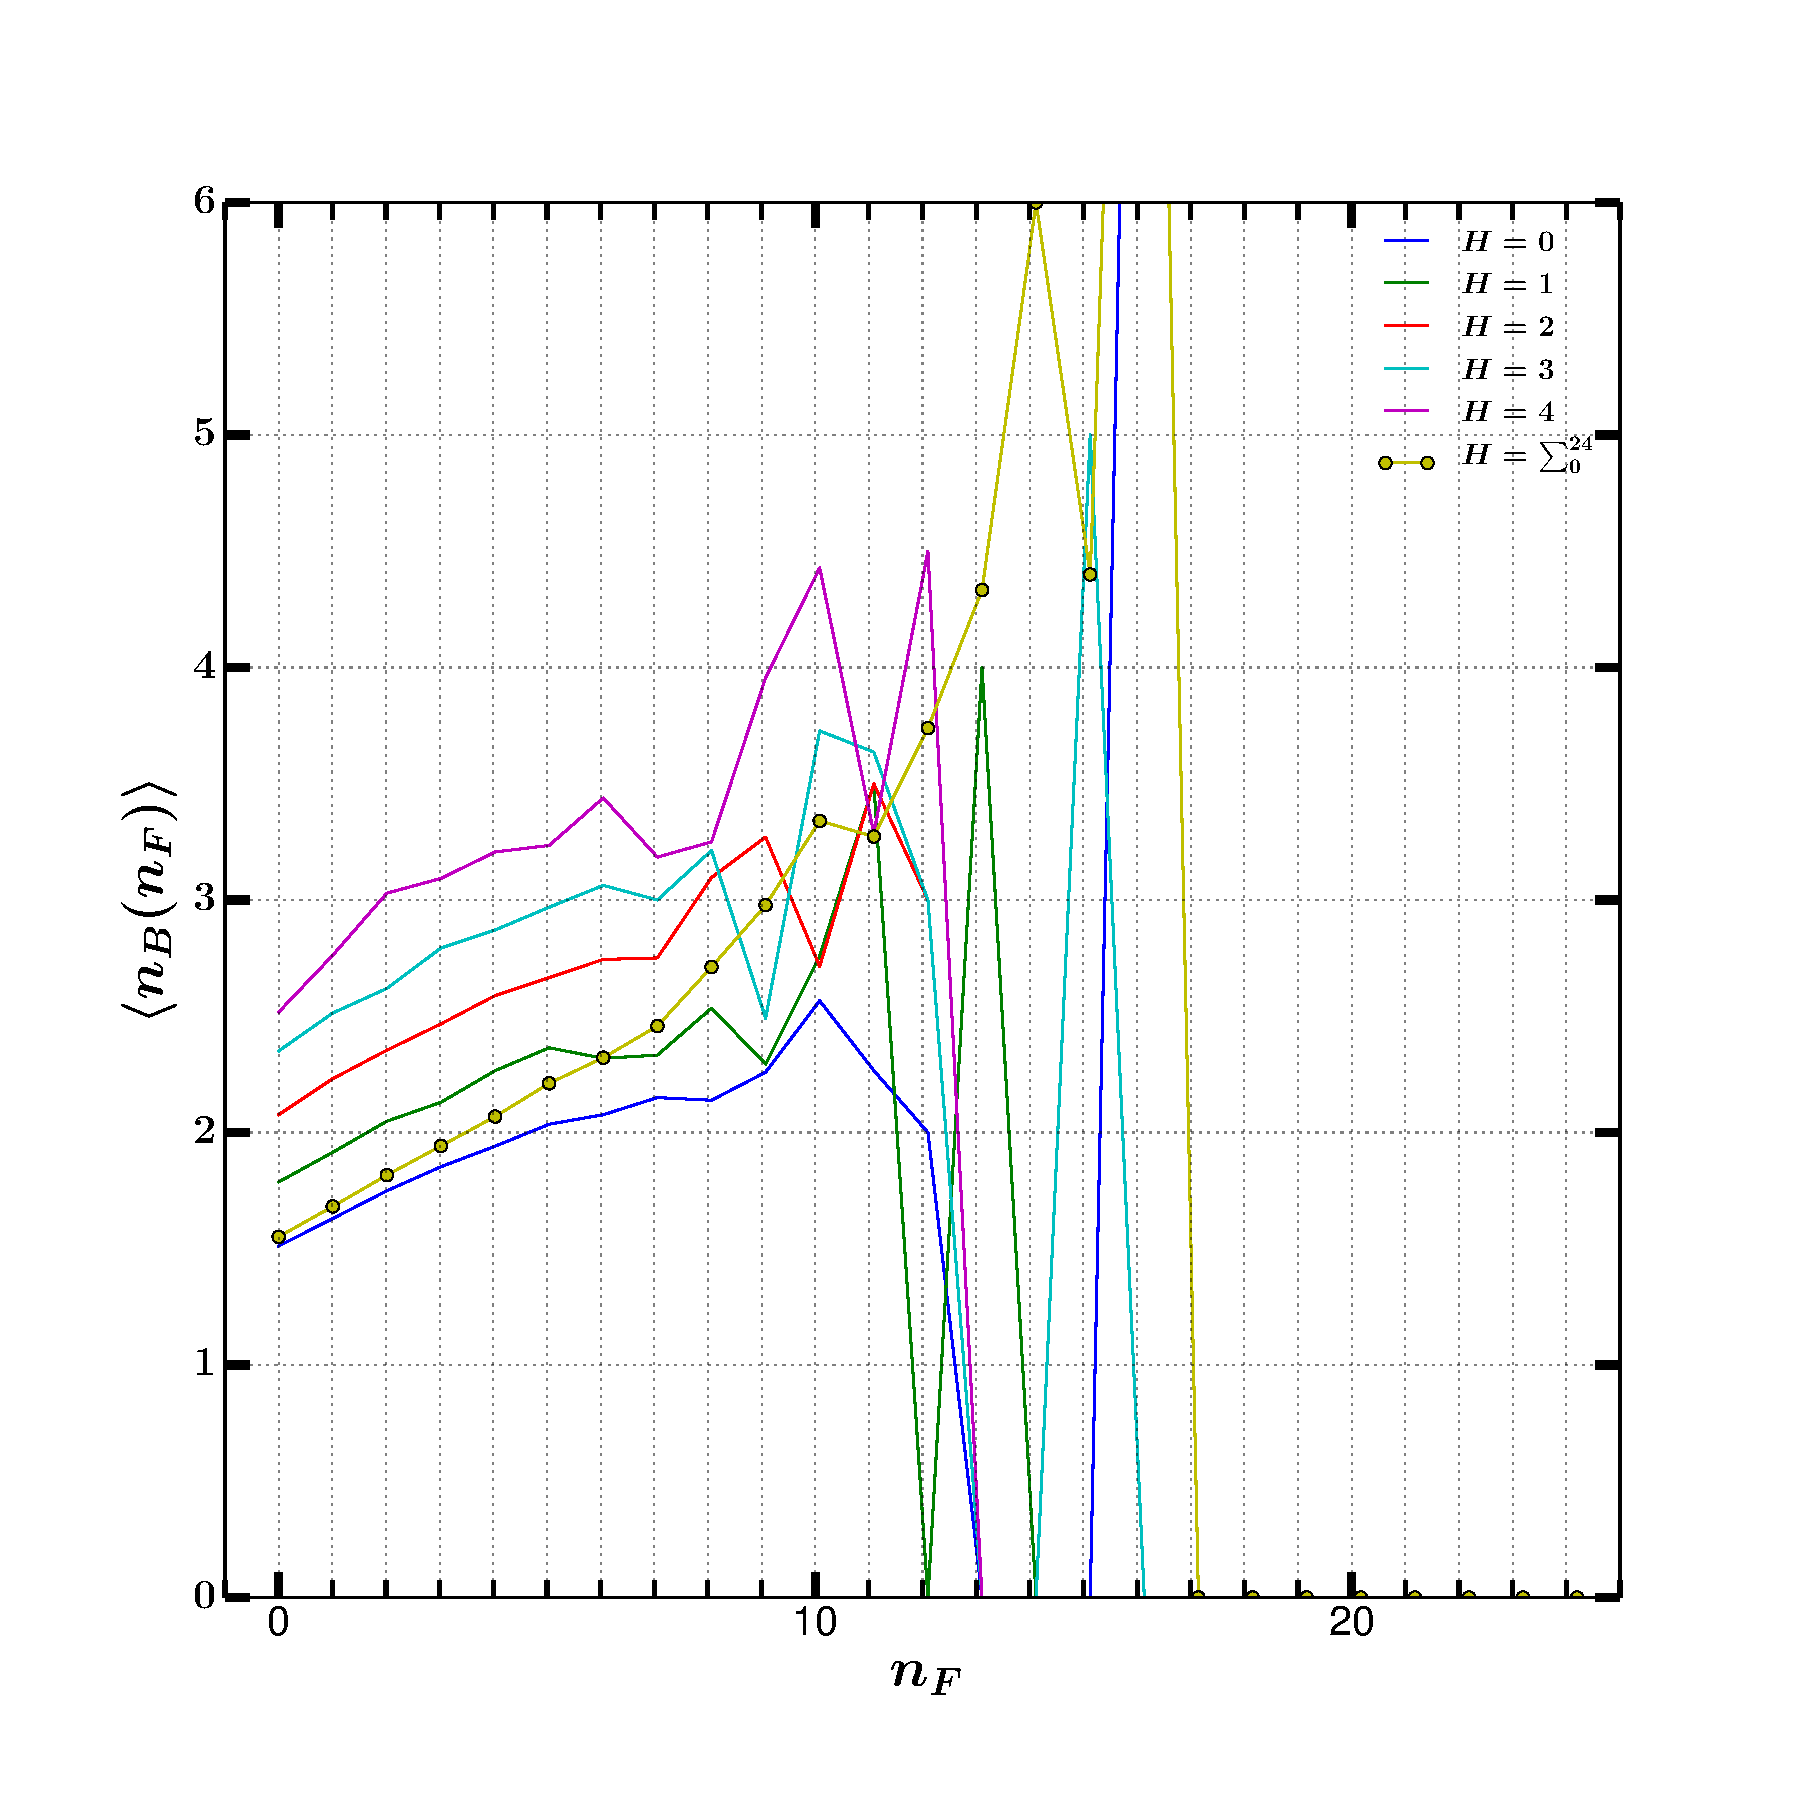
\includegraphics[scale=0.5]{../analyzed/nbnf_fixed_s_var_h.pdf}
    \caption{}
\end{figure}

\section*{\centering Non-Single diffraction, all diagrams except 1,4,6 and 10}

\end{document}
